

\chapter{System parameters}

\begin{table}[tbp]
	\centering
	\caption{Parameters and values.}
	\begin{tabular}{llll}
		\toprule
		Symbol & Parameter & Value & Unit \\
		\midrule
		$l_a$ & Distance from elevation axis to helicopter body & $0.63$  & m               \\
		$l_h$ & Distance from pitch axis to motor               & $0.18$  & m               \\
		$K_f$ & Force constant motor                            & $0.25$  & N / V            \\
		$J_e$ & Moment of inertia for elevation                 & $0.83$  & kg ${\text{m}^2}$ \\
		$J_t$ & Moment of inertia for travel                    & $0.83$  & kg ${\text{m}^2}$ \\
		$J_p$ & Moment of inertia for pitch                     & $0.034$ & kg ${\text{m}^2}$\\
		$m_h$ & Mass of helicopter                              & $1.05$  & kg              \\
		$m_w$ & Balance weight                                  & $1.87$  & kg              \\
		$m_g$ & Effective mass of the helicopter                & $0.05$  & kg              \\
		$K_p$ & Force to lift the helicopter from the ground    & $0.49$  & N               \\
		\bottomrule
	\end{tabular}
\label{tab:parameters}
\end{table}


\chapter{Simplification of helicopter model}\label{ch:linear_heli_model}


The linear approximation of the function $y = f(x,u)$ about $(x^*, u^*)$ using the first-order Taylor series and defining the new states $\Delta x = (x - x^*), \Delta u = (u-u^*)$ is defined as, 

\begin{equation}\label{eq:lin_approx}
    \begin{split}
        y &\approx f(x^*, u^*) + \frac{\partial f }{\partial x}|_{(x^*, u^*)} \Delta x + \frac{\partial f}{\partial u}|_{(x^*, u^*)} \Delta u \: \: .\\
    \end{split}
\end{equation}

Given the non-linear equations of motions of the helicopter system,
\begin{equation}
    \begin{split}
        \ddot \lambda &= -\frac{1}{J_{\lambda}}(L_3 V_s \cos e \sin p) \: \: , \\
        \ddot p &= \frac{L_1 V_d}{J_p} \: \: , \\
        \ddot e &= -\frac{1}{J_e}(L_2 \cos e + L_3 V_s \cos p) \: \: ,\\ 
    \end{split}
\end{equation}

the linear approximation described above can be used to obtain a linear approximation, which is needed for the \acrshort{mpc}-problem. 

In addition, the resulting linear system should be a first-order system, so let the states be 
\begin{equation}
    x^\top = \m{\lambda & \dot \lambda & p & \dot p & e & \dot e} \: \: ,
\end{equation}
while the inputs are 
\begin{equation}
    u^\top = \m{V_s & V_d} \: \: .
\end{equation}



\begin{equation}
    \dot x = f(x,u) = \m{\dot \lambda \\ -\frac{1}{J_{\lambda}}(L_3 V_s \cos e \sin p) \\ \dot p \\ \frac{L_1 V_d}{J_p} \\ \dot e \\ -\frac{1}{J_e}(L_2 \cos e + L_3 V_s \cos p } \: \: .
\end{equation}

The equilibrium point of the system $x^* = 0, \dot x^* = 0, \ddot x^* = 0$. This results in the input $V_s^* = -\frac{L_2}{L_3}, V_d^* = 0$. The resulting linearization becomes

\begin{equation}
    \begin{split}
        \dot x &= Ax + Bu \: \:  \\
         A &= \m{0 & 1 & 0 & 0 & 0 & 0 \\
              0 & 0 & \frac{L_2}{J_{\lambda}} & 0 & 0 & 0 \\
              0 & 0 & 0 & 1 & 0 & 0 \\
              0 & 0 & 0 & 0 & 0 & 0 \\
              0 & 0 & 0 & 0 & 0 & 1 \\
              0 & 0 & 0 & 0 & 0 & 0}, \: \: B = \m{0 & 0 \\
              0 & 0 \\
              0 & 0 \\
              0 & \frac{L_1}{J_p} \\
              0 & 0 \\
              \frac{L_3}{J_e} & 0} \: \: .
    \end{split}
\end{equation}

This is the lowest level of control. On top of this, a PD and a PID controller are added to control the pitch and elevation respectively.

\begin{equation}
    \begin{split}
        V_d = K_{pp} (p_c - p) - K_{pd} \dot p \\
        V_s = K_{ep}(e_c - e)  - K_{ed} \dot e
    \end{split}
\end{equation}

Let $u^\top = \m{p_c & e_c}$, and the  resulting first order \textit{discrete} linear system with time step $h$ is,
\begin{equation}
    \begin{split}
        \dot x &= Ax + Bu \: , \; \; \\
        A &= \m{1 & h & 0 & 0 & 0 & 0 \\
                0 & 1 & -hK_2 & 0 & 0 & 0 \\
                0 & 0 & 1 & h & 0 & 0 \\
                0 & 0 & -hK_1 K_{pp} & 1-hK_1 K_{pd} & 0 & 0 \\
                0 & 0 & 0 & 0 & 1 & h \\
                0 & 0 & 0 & 0 & -hK_3 K_{ep} & 1-hK_3 K_{ed}}, \\
        B &= \m{0 & 0 \\ 0 & 0 \\ 0 & 0 \\
                hK_1 K_{pp} & 0 \\ 0 & 0 \\ 0 & h K_3 K_{ep}} \: \: .
    \end{split}
\end{equation}


$J_e \ddot e = l_a K_f V_s - T_g.$
Mens jeg har 
$J_e \ddot e = -L_2 \cos e + L_3 V_s \cos p$




\chapter{MATLAB Code}

\begin{lstlisting}[caption={init.m}]]
% Updated spring 2018, Andreas L. Fl\r{a}ten
% Updated Spring 2019, Joakim R. Andersen

travel_gain = 1; %

%% Physical constants
m_h = 0.4; % Total mass of the motors.
m_g = 0.03; % Effective mass of the helicopter.
l_a = 0.65; % Distance from elevation axis to helicopter body
l_h = 0.17; % Distance from pitch axis to motor

% Moments of inertia
J_e = 2 * m_h * l_a *l_a;         % elevation
J_p = 2 * ( m_h/2 * l_h * l_h);   % pitch
J_t = 2 * m_h * l_a *l_a;         % travel

% Identified voltage sum and difference
V_s_eq = 6.3; % Identified equilibrium voltage sum.
V_d_eq = 0.35; % Identified equilibrium voltage difference.

% Model parameters
K_p = m_g*9.81; % Force to lift the helicopter from the ground.
K_f = K_p/V_s_eq; % Force motor constant.
K_1 = l_h*K_f/J_p;
K_2 = K_p*l_a/J_t;
K_3 = K_f*l_a/J_e;
K_4 = K_p*l_a/J_e;

%% Pitch closed loop syntesis
% Controller parameters
w_p = 1.8; % Pitch controller bandwidth.
d_p = 1.0; % Pitch controller rel. damping.
K_pp = w_p^2/K_1;
K_pd = 2*d_p*sqrt(K_pp/K_1);
Vd_ff = V_d_eq;

% Closed loop transfer functions
Vd_max = 10 - V_s_eq; % Maximum voltage difference
deg2rad = @(x) x*pi/180;
Rp_max = deg2rad(15); % Maximum reference step
s = tf('s');
G_p = K_1/(s^2);
C_p = K_pp + K_pd*s/(1+0.1*w_p*s);
L_p = G_p*C_p;
S_p = (1 + L_p)^(-1);

%% Elevation closed loop analysis
% Controller parameters
w_e = 0.5; % Elevation controller bandwidth.
d_e = 1.0; % Elevation controller rel. damping.
K_ep = w_e^2/K_3;
K_ed = 2*d_e*sqrt(K_ep/K_3);
K_ei = K_ep*0.1;
Vs_ff = V_s_eq;

% Closed loop transfer functions
Vs_max = 10 - V_s_eq; % Maximum voltage sum
Re_max = deg2rad(10); % Maximum elevation step
G_e = K_3/(s^2);
C_e = K_ep + K_ed*s/(1+0.1*w_e*s) + K_ei/s;
L_e = G_e*C_e;
S_e = (1 + L_e)^(-1);
\end{lstlisting}




\begin{lstlisting}[caption={data.m}]]
% system: x+ = Ax + Bu + Ew
% constraints: Z = {x, u | Cx + Du \leq e }
% disturbance parameters: Mw \leq g

%horizon
system.N = 15;

% system 
system.h=0.08;
A = [0 1    0        0       0        0;
     0 0 -K_2        0       0        0;
     0 0    0        1       0        0;
     0 0 -K_1*K_pp -K_1*K_pd 0        0;
     0 0    0        0       0        1;
     0 0    0        0  -K_3*K_ep -K_3*K_ed];
B =    [0           0;
        0           0;
        0           0;
        K_1*K_pp    0;
        0           0;
        0        K_3*K_ep];

%disturbance
E = [1;0;0;0;0;0;0;0];    

A_d = [1;0;0;0;0;0];

A_e = [0;0;0;0;0;0;0];

%discretize helicopter equations   
system.A_heli = system.h * A + eye(size(A,1));
system.B_heli = system.h * B;    
system.E = system.h * E;

%system with offset
system.A_offset = [system.A_heli A_d; ...
            zeros(1,size(A,1)) 1];
system.B_offset = [system.B_heli; 0 0];    
system.A = [system.A_offset A_e; ...
            zeros(1, size(system.A_offset,1)+1)];
system.B = [system.B_offset; 0 0];

system.n = size(system.A,2);
system.m = size(system.B,2);

% for estimator
system.C_offset = [eye(system.n-2) zeros(system.n-2, 1)];
system.C = [system.C_offset zeros(system.n-2, 1)];
system.D = zeros(system.n, system.m);


%constraints
lambda_lim = 210 * DEGTORAD;
lambda_rate_lim = 1000000;
p_lim = 30 * DEGTORAD;
p_rate_lim = 1000000;
e_lim = 1000000;
e_rate_lim = 10000;
u_1_lim = 25 * DEGTORAD;
u_2_lim = 1000000;
constraints.C = [1 0 0 0 0 0 0 0; 
                 -1 0 0 0 0 0 0 0; 
                 0 1 0 0 0 0 0 0;  
                 0 -1 0 0 0 0 0 0;
                 0 0 1 0 0 0 0 -1; %slack - soft constraint
                 0 0 -1 0 0 0 0 -1;  %slack - soft constraint
                 0 0 0 1 0 0 0 0; 
                 0 0 0 -1 0 0 0 0;
                 0 0 0 0 1 0 0 0; 
                 0 0 0 0 -1 0 0 0; 
                 0 0 0 0 0 1 0 0; 
                 0 0 0 0 0 -1 0 0;
                 0 0 0 0 0 0 0 -1;
                 0 0 0 0 0 0 0 0; 
                 0 0 0 0 0 0 0 0;
                 0 0 0 0 0 0 0 0; 
                 0 0 0 0 0 0 0 0];
constraints.D = [0 0; 
                 0 0; 
                 0 0; 
                 0 0; 
                 0 0; 
                 0 0; 
                 0 0; 
                 0 0; 
                 0 0; 
                 0 0; 
                 0 0; 
                 0 0; 
                 0 0;
                 1 0; 
                 -1 0; 
                 0 1; 
                 0 -1];
constraints.e = [lambda_lim; 
                 lambda_lim; 
                 lambda_rate_lim; 
                 lambda_rate_lim;
                 p_lim; 
                 p_lim; 
                 p_rate_lim;
                 p_rate_lim;
                 e_lim; 
                 e_lim; 
                 e_rate_lim; 
                 e_rate_lim;  
                 0; %slack
                 u_1_lim; 
                 u_1_lim; 
                 u_2_lim;
                 u_2_lim];
             
% disturbance
% used when simulating the disturbance
disturbance.E = [1; -1];
dist_low_bd = 1.1459;
dist_up_bd = 1.4324;
disturbance.g = [dist_up_bd * DEGTORAD; -dist_low_bd * DEGTORAD];
\end{lstlisting}



\begin{lstlisting}[caption={exe\_sim.m}, label={lst:exe_sim}]
set(groot, 'defaultAxesTickLabelInterpreter','latex'); set(groot, 'defaultLegendInterpreter','latex');
set(0,'defaultTextInterpreter','latex'); %trying to set the default

clear x u v z
%% loading
system.Nsim = 400;
%system.stable = 1;
%with_estimator = 1;
%slack_var = 1;
DEGTORAD = pi/180;
init;
data;
%% tune MPC
% cost
%cost of slack
s = 0.3;
Q_vec = [3 2 1 1 2 1];
cost.Q_heli = diag(Q_vec);
cost.Q = diag([Q_vec 0 s]); %slack weight
cost.R = diag([1.5 1]);

offline_calc_osqp;

%% disturbance
% problem.system.w_sequence = generate_disturbance(problem);
w_sequence = generate_disturbance(problem);
problem.system.w_sequence = w_sequence;

travel_offset = 50;
elevation_offset = 30;
system.x0 = [-travel_offset*DEGTORAD; 0; 0; 0; -elevation_offset * DEGTORAD; 0; 0; 0];

%clear z u x v
x(:,1) = system.x0;
x_est(:,1) = system.x0;
%% 
gen_code_osqp;
gen_code_params;

%qc_build_model('helicopter_mpc')

%%
sim = 0;
if(sim)
for i = 1:system.Nsim
    %state estimator
   
    % Return optimal u for horizon
    if (with_estimator==1)
        if (slack_var)
            optimal(i) = online_calc(problem,x_est(:,i));
        else
            optimal(i) = online_calc_osqp(problem,x_est(:,i));
        end
        v(:,i) = optimal(i).v(:,1);
        z(:,i) = optimal(i).z(:,1);
        e(i) = optimal(i).e;
        u(:,i) = v(:,i);
        x_est(:,i+1) = problem.system.A * x_est(:,i) + problem.system.B * u(:,i) + L' * system.C * (x(:,i) - x_est(:,i));
    else
        if (slack_var)
            optimal(i) = online_calc(problem,x(:,i));
        else
            optimal(i) = online_calc_osqp(problem,x(:,i));
        end
        v(:,i) = optimal(i).v(:,1);
        z(:,i) = optimal(i).z(:,1);
        e(i) = optimal(i).e;
        u(:,i) = v(:,i);        
    end
    
    if ~(i == system.Nsim)
        x(:,i+1) = problem.system.A * x(:,i) + problem.system.B * u(:,i) ...
            + problem.system.E * problem.system.w_sequence(:,i);
    end
end
end


%% PLOTTING
close all 

%plot_sim;

% if (with_estimator)
%     plot_error;
% end
% plot_heli;
\end{lstlisting}

\begin{lstlisting}[caption={offline\_calc.m}, label={lst:offline_calc}]
% state feedback and terminal cost
[K, P] = dlqr(system.A_heli, system.B_heli, cost.Q_heli, cost.R);

% extend to add system state d
system.K = [-K zeros(system.m, 2)];
cost.P = [P zeros(size(P,1), 2) ;
          zeros(2, size(P,1)+2)];
cost.P(system.n, system.n) = 1;      
      
system.A_K = system.A + system.B * system.K; 
constraints.C_K = constraints.C + constraints.D * system.K;
% generate matrices for MPC without eq.constr.
[Sx, Su] = genMPCprob(system.A,system.B,system.N);
system.Sx = Sx;
system.Su = Su;

%terminal constraint set 
[X_tc , d_index] = terminal_constraint(system,constraints);
%[X_tc_3 , d_index_3] = terminal_constraint_3(system,constraints, system.N);
%X_tc = terminal_constraint_2(system,constraints);
constraints.G = X_tc.A;
constraints.h = X_tc.b;
   
% generate state estimator gain L
%these are randomly selected

p = [0.3; 
     0.4; 
     0.5 + 0.15i; 
     0.5 - 0.15i; 
     0.52 + 0.05i; 
     0.52 - 0.05i; 
     0.6];

L_offset = place(system.A_offset', system.C_offset', p);

L = [L_offset zeros(system.n-2, 1)];

%assign to problem
problem.system = system;
problem.constraints = constraints;
problem.cost = cost;
problem.disturbance = disturbance;

% generate mpc matrices
if (slack_var)
    [problem.mpc_cost, problem.mpc_constraints] = generate_mpc_matrices(problem);
else    
    [problem.mpc_cost, problem.mpc_constraints] = generate_mpc_matrices_osqp(problem);
end   
\end{lstlisting}

\begin{lstlisting}[caption={generate\_mpc\_matrices.m}, label={lst:gen_mpc}]
function [mpc_cost, mpc_constraints] = generate_mpc_matrices(problem)

N = problem.system.N;
n = problem.system.n;
m = problem.system.m;
% Inequality constraints

% Cx + Du \leq e
% Gx_N \leq h
C_bar = kron(eye(N), problem.constraints.C);
D_bar = kron(eye(N), problem.constraints.D);
e_bar = kron(ones(N,1),problem.constraints.e);
G_bar = [zeros(size(problem.constraints.G,1) , n * (N-1)) problem.constraints.G ];

a = [C_bar; 
     G_bar];
b = [D_bar; zeros(size(problem.constraints.G,1) , m * N) ];
c = [e_bar; problem.constraints.h];

if (problem.system.stable)
    mpc_constraints.Ain = [a b];
    mpc_constraints.bin = [c];
else
    mpc_constraints.Ain = [C_bar D_bar];
    mpc_constraints.bin = [e_bar];
end
% Equality constraints

mpc_constraints.Aeq = gen_aeq(problem.system.A, problem.system.B, N, n, m);
mpc_constraints.beq = [problem.system.A; zeros((N-1)*n, n) ];

% Cost
if (problem.system.stable)
    H = blkdiag(kron(eye(problem.system.N-1), problem.cost.Q), problem.cost.P, ...
            kron(eye(problem.system.N), problem.cost.R));
else        
    H = blkdiag(kron(eye(problem.system.N), problem.cost.Q), ...
            kron(eye(problem.system.N), problem.cost.R));
end        
mpc_cost.H = 2*H;
mpc_cost.f = zeros(size(H,1), 1);
\end{lstlisting}

\begin{lstlisting}[caption={generate\_mpc\_matrices\_osqp.m}, label={lst:gen_mpc_osqp}]
function [mpc_cost, mpc_constraints] = generate_mpc_matrices_osqp(problem)

N = problem.system.N;
n = problem.system.n;
m = problem.system.m;
Sx = problem.system.Sx;
Su = problem.system.Su;
%x = Su * u + Sx * x0


% Inequality constraints

% Cx + Du \leq e
C_bar = kron(eye(N), problem.constraints.C);
D_bar = kron(eye(N), problem.constraints.D);
a1 = C_bar * Su + D_bar;
b1 = kron(ones(N,1),problem.constraints.e);
c1 =  -C_bar * Sx;

% GzN \leq h

a2 = problem.constraints.G * Su((N-1)*n+1:end, 1:end);
b2 = problem.constraints.h;
c2 = -problem.constraints.G * Sx((N-1)*n+1:end,1:n);

if (problem.system.stable)
    mpc_constraints.Ain = [a1; a2];
    mpc_constraints.bin = [b1; b2];
    mpc_constraints.cin = [c1; c2];
else
    mpc_constraints.Ain = a1;
    mpc_constraints.bin = b1;
    mpc_constraints.cin = c1;
end
% Cost

if(problem.system.stable)
    Q_big = blkdiag(kron(eye(N-1), problem.cost.Q), problem.cost.P);
else
    Q_big = blkdiag(kron(eye(N), problem.cost.Q));
end    

R_big = kron(eye(problem.system.N), problem.cost.R);
H = Su' * Q_big * Su + R_big;
f = 2 * Sx' * Q_big * Su;

mpc_cost.H = 2 * H;
mpc_cost.f = f;
\end{lstlisting}

\begin{lstlisting}[caption={online\_calc.m}, label={online_calc}]
function optimal = online_calc_osqp(problem,x)

N = problem.system.N;
n = problem.system.n;
m = problem.system.m;

% get optimal decision variable and optimal value
% OSQP: min 0.5 x' * H * x + (x_0' * f)' * x
%      s.t Ain \leq bin + cin * x0
%          [C C C ... C] X + [D D D ... D] U \leq [e e e ... e]'
%          [C C C ... C] (Su * U + Sx * x0) + [D D D ... D] U \leq [e e e ... e]'
%          G x_N \leq h

H = problem.mpc_cost.H;
f = problem.mpc_cost.f;
q = (x' * f)';
A = problem.mpc_constraints.Ain;
bin = problem.mpc_constraints.bin;
cin = problem.mpc_constraints.cin;

ub = bin + cin * x;
lb = -Inf * ones(size(ub,1),1); 

qp_problem = osqp;
settings = qp_problem.default_settings();
settings.eps_abs = 1e-04;
settings.eps_rel = 1e-04;
settings.verbose = 0;

qp_problem.setup(H, ...
                 q, ...             
                 A, lb, ub, ...
                 settings);             
output = qp_problem.solve();

% x^+ = Su u * Sx * x0

z = zeros(n,N);
v = zeros(m,N);
%display(output.x(1));
z_tmp = problem.system.Su * output.x + problem.system.Sx * x;
v_tmp = output.x;
for i = 1:problem.system.N
    z(:,i) = z_tmp((i-1)*n + 1:i*n);
    v(:,i) = v_tmp((i-1)*m + 1:i*m);
end    

optimal.z = z;
optimal.v = v;
optimal.e = output.info.status_val;

\end{lstlisting}

\begin{lstlisting}[caption={genMPCprob.m}, label={lst:genMPCprob}]
function [Sx Su] = genMPCprob(A,B,N)

% Generate reduced space matrices for MPC QP problem
% Inputs: 
%   A, B        System matrices in discrete time system: x+ = A x + B u
%   N           Control horizon length (degrees of freedom)
% 
% Outputs:
%   Sx          State predictions: 
%   Su              [x_1 x_2 ... x_N] = Sx*x_0 + Su*[u_0 u_1 ... u_N-1]

% 12/02/2018 Lars Imsland

% Define predictions:
% [x_1 x_2 ... x_N] = Sx*x_0 + Su*[u_0 u_1 ... u_N-1]

nx = size(A,1);
nu = size(B,2);

Sx = [eye(nx);A];
Su = zeros(N*nx,N*nu);
Su(1:nx,1:nu) = B;
for i = 2:N,
    Sx = [Sx;Sx((i-1)*nx+1:i*nx,:)*A];
    for j=1:i,
        Su((i-1)*nx+1:i*nx,(j-1)*nu+1:j*nu) = ...
            Sx((i-j)*nx+1:(i-j+1)*nx,1:nx)*B;
    end
end
Sx = Sx(nx+1:end,:); % remove first I
\end{lstlisting}

\begin{lstlisting}[caption={gen\_aeq.m}, label={lst:gen_aeq}]
function A = gen_aeq(A1,B1,N,mx,mu)
% Function to build a matrix representing equality constraints for a 
% linear discrete time dynamical system. The resulting matrix has the form                            
%      -                    -                                   
%      |I        |-B1       |                                   
%  A = |-A1 I    |  -B1     |                                   
%      |   . .   |     .    |                                   
%      |   -A1 I |      -B1 |                                   
%      -                    -                                   
%                                                               
% A1 - Discrete time system matrix                          
% B1 - Discrete time input matrix                       
% N  - Time horizon, assumes M = N
% mx - Number of states                               
% mu - Number of inputs                                     
%                                                               
% 08.03.2001 Geir Stian Landsverk
% January 2018, Andreas L. Fl\r{a}ten (translation to English)
                                                              

A 	= zeros(N*mx,N*mx+N*mu);
b1 = diag_repeat(-B1, N);
a1	= eye(N*mx);
for i=1:(N-1)
  a1([(i*mx+1):((i+1)*mx)],[((i-1)*mx+1):(i*mx)])=-A1;
end
A	= [a1 b1];
\end{lstlisting}

\begin{lstlisting}[caption={diag\_repeat.m}, label={lst:diag_repeat}]
function y = diag_repeat(varargin)

% BLKDIAG2  Block diagonal concatenation of input arguments.
%
%                                   |A 0 .. 0|
%   Y = diag_repeat(A,N)  produces  |0 A .. 0|
%                                   |0 0 .. A|
%   where 	size(A) = [m,n]
%			size(Y) = [N*m,N*n]
%
%   See also DIAG, HORZCAT, VERTCAT

% Wes Wang 9/9/94, 9/30/95.  Greg Wolodkin 1/30/98
% Copyright (c) 1984-98 by The MathWorks, Inc.
% $Revision: 1.2 $

% Modified version of blkdiag.m
% Geir Stian Landsverk 3/8/01


x = varargin{1};
[p2,m2] = size(x);
y = [];
for k = 1:varargin{2}
  [p1,m1] = size(y); 
  y = [y zeros(p1,m2); zeros(p2,m1) x];
end
\end{lstlisting}



\chapter{Simulink model}%\label{sec:simulink_model_pic}

\begin{figure}
    \centering
    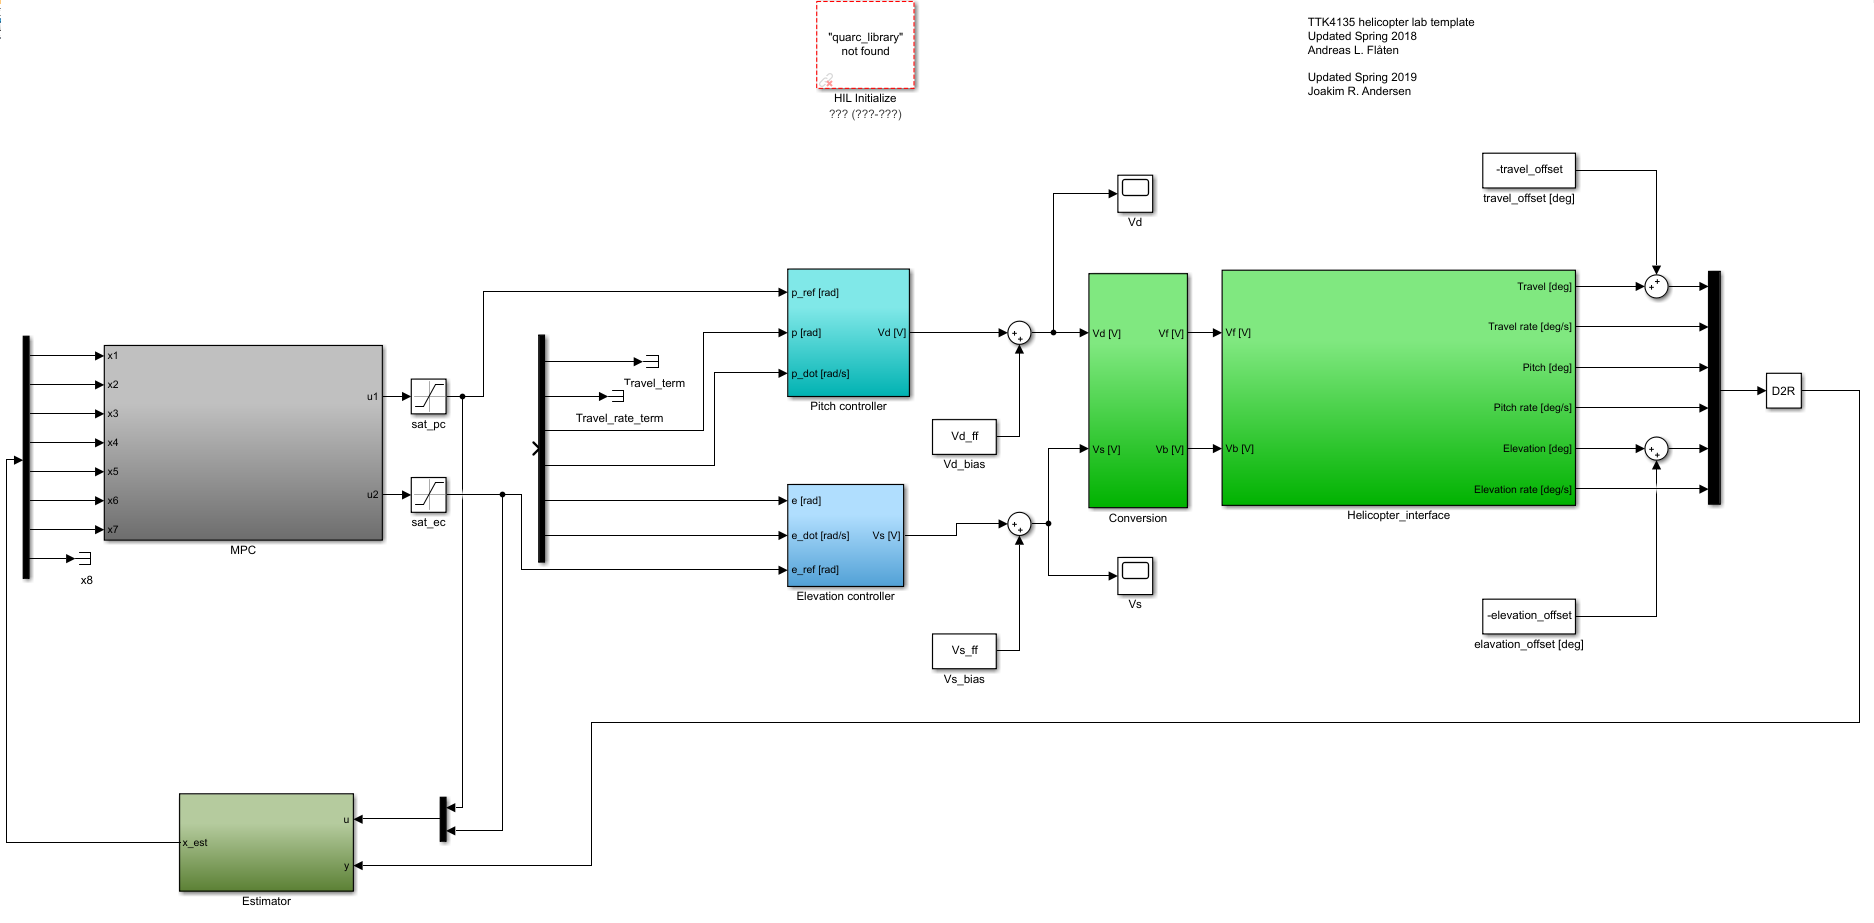
\includegraphics[angle=90,origin=c, scale=0.4]{fig/simulink/system.png}
    \caption{Simulink model}
    \label{fig:simulink_system}
\end{figure}

\begin{figure}
    \centering
    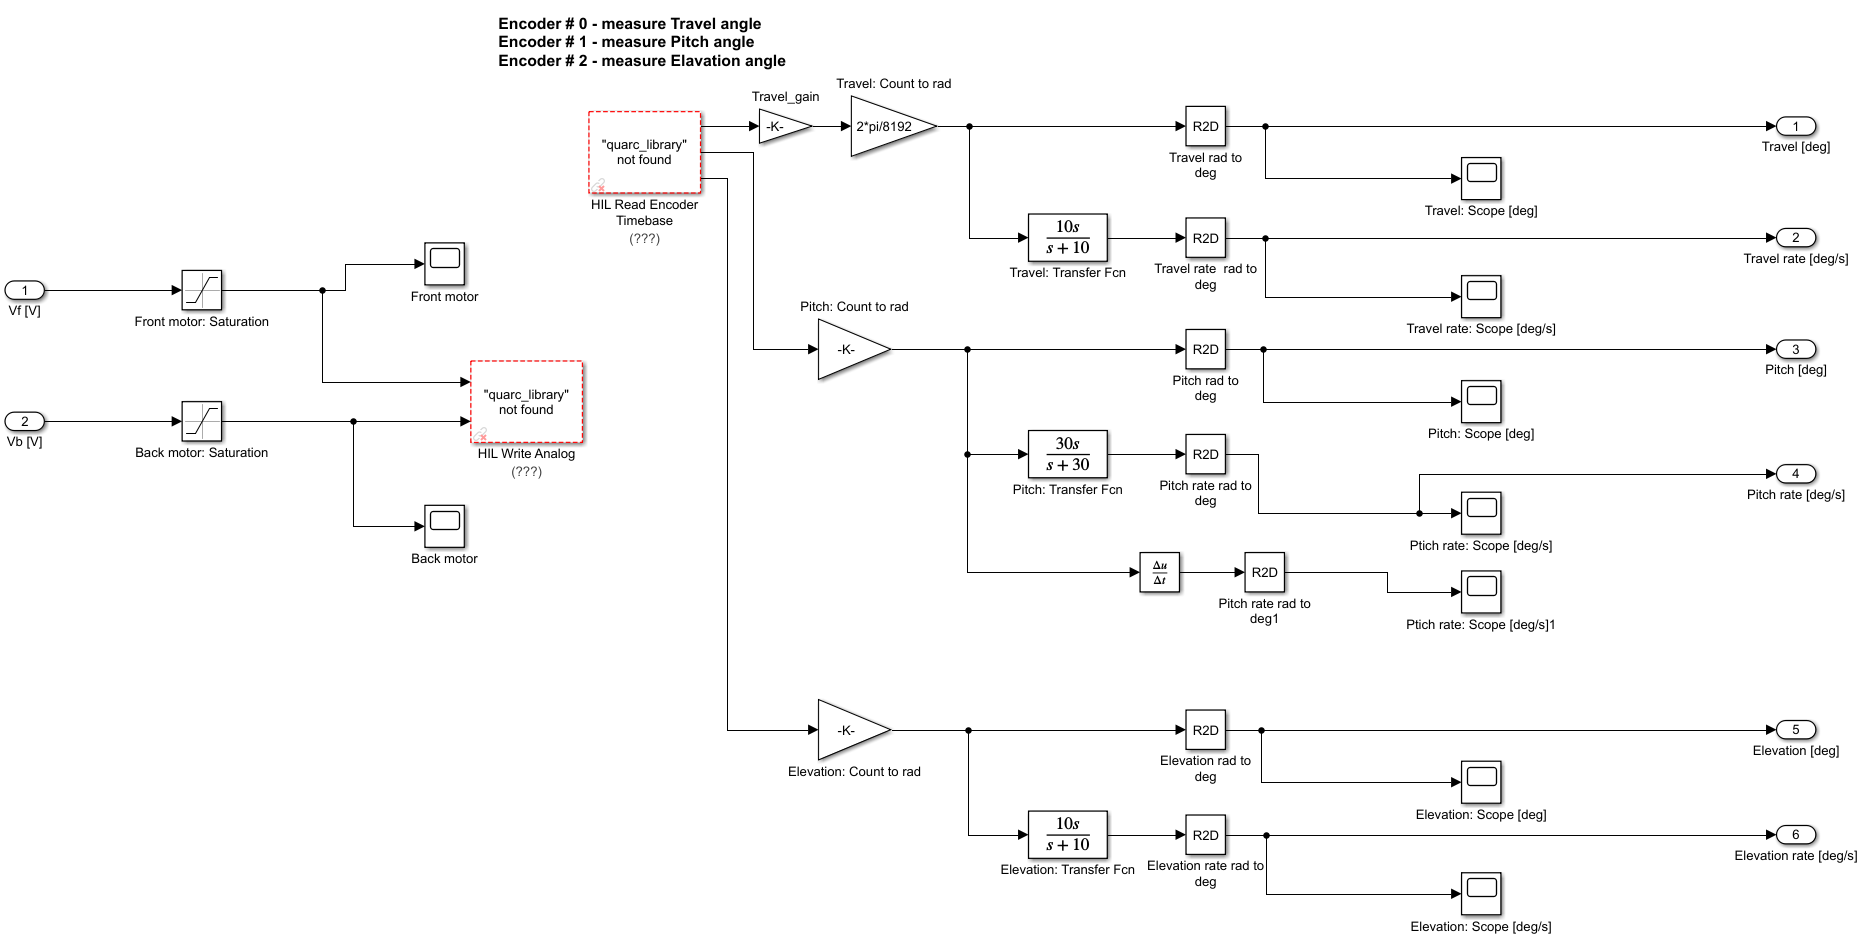
\includegraphics[scale=0.20]{fig/simulink/heli_interface.png}
    \caption{Helicopter interface}
    \label{fig:simulink_heli_interface}
\end{figure}

\begin{figure}
    \centering
    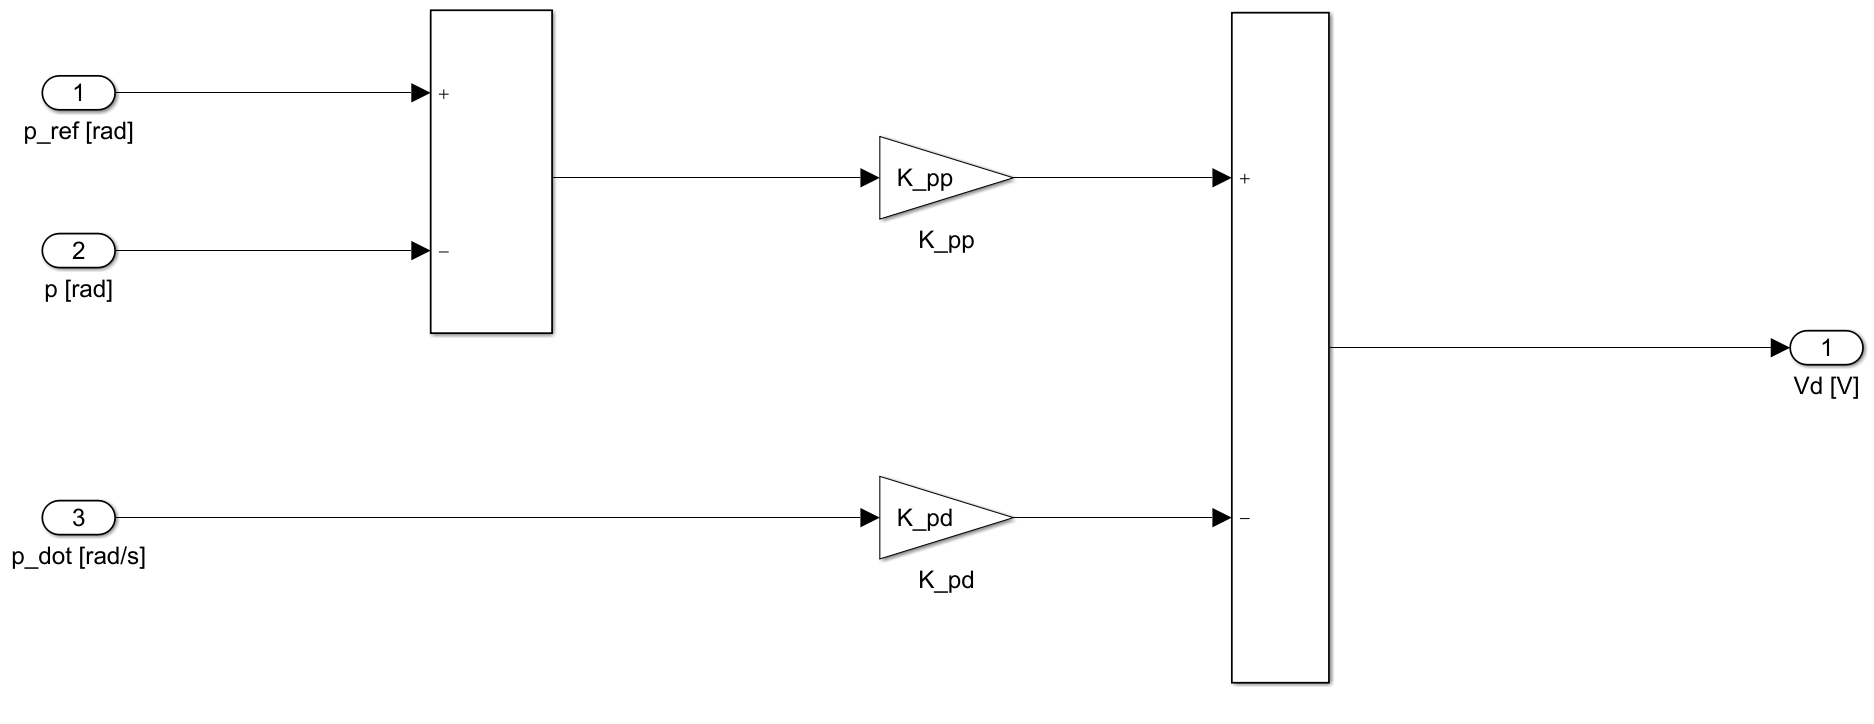
\includegraphics[scale=0.2]{fig/simulink/pitch_controller.png}
    \caption{Pitch controller}
    \label{fig:simulink_pitch_contr}
\end{figure}

\begin{figure}
    \centering
    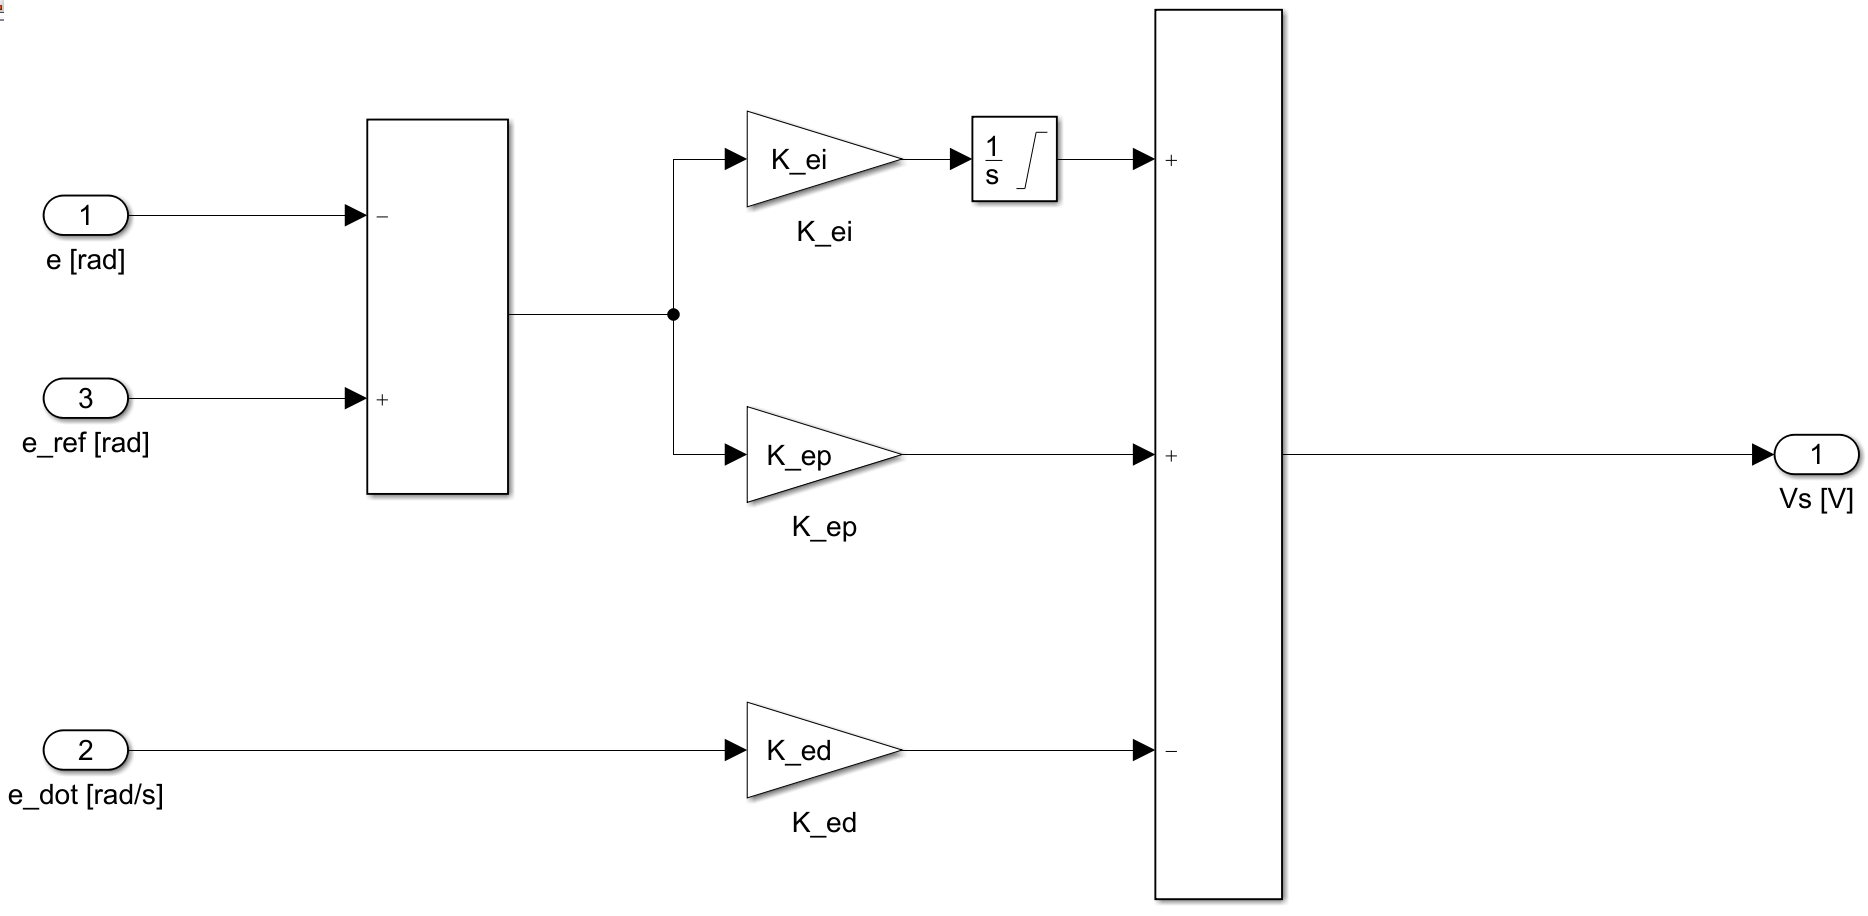
\includegraphics[scale=0.2]{fig/simulink/elevation_controller.png}
    \caption{Elevation controller}
    \label{fig:simulink_elev_contr}
\end{figure}

\begin{figure}
    \centering
    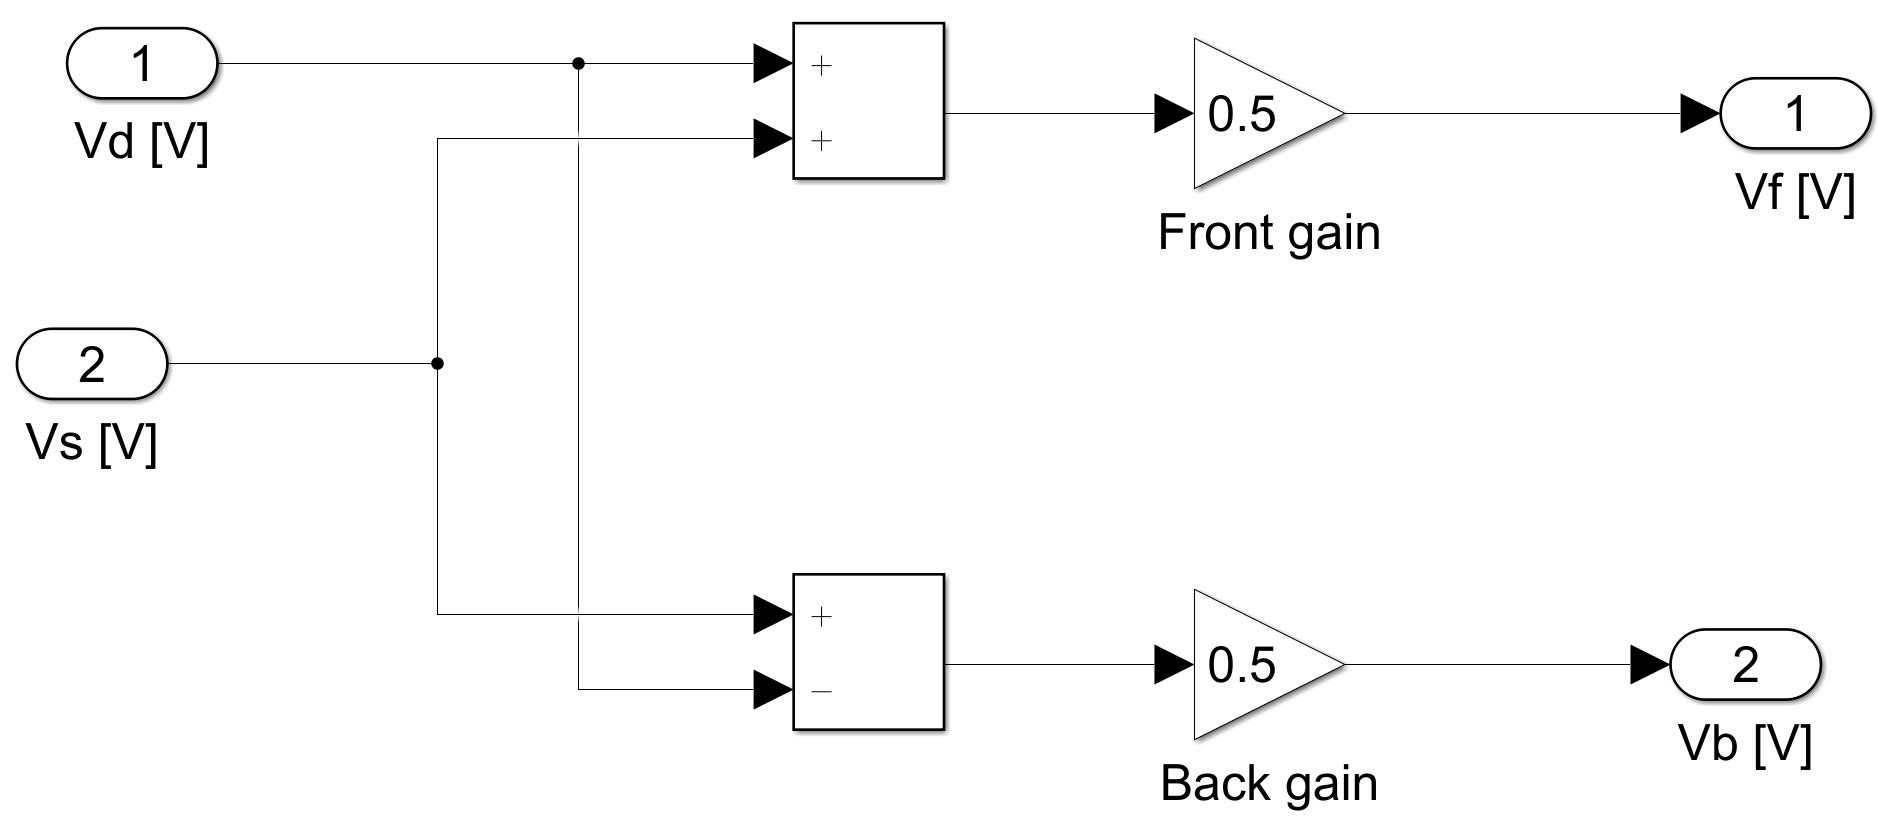
\includegraphics[scale=0.2]{fig/simulink/Vd_Vs_block.png}
    \caption{Voltage conversion block}
    \label{fig:simulink_Vd_Vs_block}
\end{figure}

\begin{figure}
    \centering
    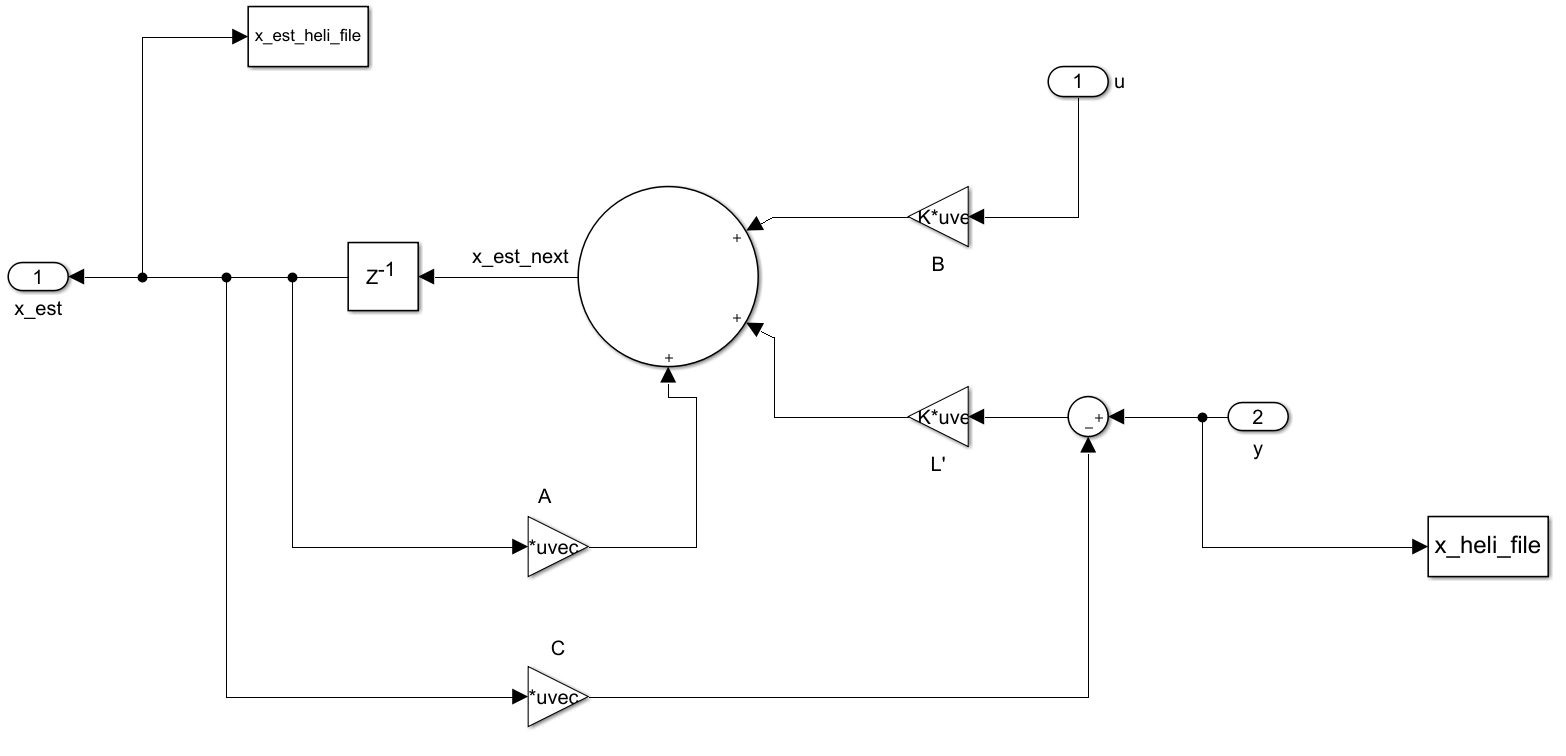
\includegraphics[scale=0.2]{fig/simulink/estimator.png}
    \caption{Estimator}
    \label{fig:simulink_estimator}
\end{figure}